\chapter{Intégration numérique}\label{chap-quadrature} 
La méthode des éléments finis conduit à la discrétisation d'une formulation faible où la construction des matrices constitutives du système à résoudre nécessitent le calcul d'intégrales. Dans certains cas particuliers, ou en utilisant des codes de calcul formel, ces intégrations peuvent être réalisées de manière exacte. Cependant, dans la plupart des cas et dans la plupart des codes de calcul, ces intégrations sont calculées numériquement. On parle alors de méthodes d'intégration numérique et de formules de quadrature. 
%%%%----------------------------------------------------------
\section{Méthodes de Newton-Cotes}\index[aut]{Cotes (Roger), 1682-1716, Anglais}\index[aut]{Newton (Isaac, Sir -), 1643-1727, Anglais}\index{intégration!méthode!de Newton-Cotes}
%%%%----------------------------------------------------------
Soit à calculer l'intégrale suivante: 
\begin{equation}
I=\int_a^b f(x)\dd x
\end{equation}
L'idée consiste à construire un polynôme pour interpoler~$f(x)$ et à intégrer ce polynôme. Plusieurs types de polynômes peuvent être utilisés pour cette interpolation. Les principales méthodes d'interpolations sont détaillées au chapitre~\ref{chap-interpolation}. 
%%%%----------------------------------------------------------
\subsection{Méthode des rectangles}\index{intégration!méthode!des rectangles}
%%%%----------------------------------------------------------
La \textcolorblue{méthode des rectangles} consiste à interpoler~$f(x)$ par un polynôme de degré~$0$, i.e. par la constante valant, selon les variantes de la méthode, soit~$f(a)$, soit~$f((a+b)/2)$. Comme cette approximation est très brutale, il est possible de subsiviser l'intervalle~$\intff{a}{b}$ en plusieurs intervalles et d'appliquer la méthode sur chacun des intervalles, i.e. d'approcher~$f$ par une fonction en escalier. Si l'on subsivise l'intervalle~$\intff{a}{b}$ en~$n$ intervalles égaux, il vient alors: 
\begin{equation}
I\approx h\sum_{i=0}^{n-1} f(x_i)
\end{equation}
où~$h=(b-a)/n$ est la longueur de chaque sous intervalle et~$x_i=a+ih$ le point courant. 
%%%%----------------------------------------------------------
\subsection{Méthode des trapèzes}\index{intégration!méthode!des trapèzes} 
%%%%----------------------------------------------------------
La \textcolorblue{méthode des trapèzes} consiste à interpoler~$f(x)$ par un polynôme de degré~$1$, i.e. par la droite passant par les points~$(a,f(a))$ et~$(b,f(b))$. On obtient alors: 
\begin{equation}
 I\approx h\dfrac{f(a)+f(b)}2
\end{equation}
où~$h=b-a$ est la longueur de l'intervalle, et l'erreur commise vaut~$-\frac{h^3}{12} f''(w)$ pour un certain~$w\in\intff{a}{b}$ (sous réserve que~$f$ soit 2 fois dérivable). L'erreur étant proportionnelle à~$f''$, la méthode est dite d'ordre~$2$, ce qui signifie qu'elle est exacte (erreur nulle) pour tout polynôme de degré inférieur où égale à 1. 

Comme cette approximation peut sembler un peu brutale, il est possible de subsiviser l'intervalle~$\intff{a}{b}$ en plusieurs intervalles et d'appliquer cette formule sur chacun des intervalles, i.e. d'approcher~$f$ par une fonction affine continue par morceaux. Si l'on subsivise l'intervalle~$\intff{a}{b}$ en~$n$ intervalles égaux, il vient alors: 
\begin{equation}
I\approx \frac{(b-a)}{n}\sum_{i=0}^{n}f(x_i)
\end{equation}
où~$h=(b-a)/n$ est la longueur de chaque sous intervalle, $x_i=a+ih$ le point courant et l'erreur commise vaut~$-\frac{h^3}{12n^2} f''(w)$ pour un certain~$w\in\intff{a}{b}$. 
\begin{remarque}[Remarques]\mbox{}
\begin{itemize}
\item la \textcolorblue{méthode de Romberg} permet d'accélérer la convergence de la méthode des trapèzes;
\item la méthode des trapèzes est une méthode de Newton-Cotes pour~$n=1$.\index[aut]{Cotes (Roger), 1682-1716, Anglais}\index[aut]{Newton (Isaac, Sir -), 1643-1727, Anglais}\index{intégration!méthode!de Newton-Cotes} 
\end{itemize}
\end{remarque} 
%%%%----------------------------------------------------------
\subsection{Méthode de Simpson}\index{intégration!méthode!de Simpson}\index[aut]{Simpson (Thomas), 1710-1761, Anglais} 
%%%%----------------------------------------------------------
La \textcolorblue{méthode de Simpson} consiste à interpoler~$f(x)$ par un polynôme de degré~$2$, i.e. par la parabole passant par les points extrêmes~$(a,f(a))$ et~$(b,f(b))$ et le point milieu~$(c,f(c))$ avec~$c=(a+b)/2$. On obtient alors: 
\begin{equation}
 I\approx \frac{h}{6} \left( f(a)+f(b)+f(c)\right)
\end{equation}
où~$h=b-a$ est la longueur de l'intervalle, et l'erreur commise vaut~$-\frac{h^5}{2^5.90} f^{(4)}(w)$ pour un certain~$w\in\intff{a}{b}$ (sous réserve que~$f$ soit quatre fois dérivable). L'erreur étant proportionnelle à~$f^{(4)}$, la méthode est dite d'ordre~$4$, ce qui signifie qu'elle est exacte (erreur nulle) pour tout polynôme de degré inférieur où égale à 3. 

Comme dans le cas précédent, il est possible de subsiviser l'intervalle~$\intff{a}{b}$ en plusieurs intervalles et d'appliquer cette formule sur chacun des intervalles. Si l'on subsivise l'intervalle~$\intff{a}{b}$ en~$n$ intervalles égaux, avec~$n$ pair, il vient alors: 
\begin{equation}
 I\approx \frac{h}{3} \left( f(a)+f(b)+2\sum_{i=1}^{n/2-1}f(x_{2i})+4\sum_{i=1}^{n/2}f(x_{2i-1}) \right)
\end{equation}
où~$h=(b-a)/n$ est la longueur de chaque sous intervalle, $x_i=a+ih$ le point courant et l'erreur commise vaut~$-\frac{nh^5}{180} f^{(4)}(w)$ pour un certain~$w\in\intff{a}{b}$. 
\begin{remarque}[Remarques]\mbox{}
\begin{itemize}
\item la parabole interpolant~$f$ est trouvée en utilisant l'interpolation de Lagrange;\index[aut]{Lagrange (Joseph Louis, comte de -), 1736-1813, Italien} 
\item la méthode de Simpson\index[aut]{Simpson (Thomas), 1710-1761, Anglais} est un cas particulier de celle de Newton-Cotes pour~$n=2$.\index[aut]{Cotes (Roger), 1682-1716, Anglais}\index[aut]{Newton (Isaac, Sir -), 1643-1727, Anglais}\index{intégration!méthode!de Newton-Cotes} 
\end{itemize}
\end{remarque}
%%%%----------------------------------------------------------
\subsection*{Méthode de Newton-Cotes}\index[aut]{Cotes (Roger), 1682-1716, Anglais}\index[aut]{Newton (Isaac, Sir -), 1643-1727, Anglais}\index{intégration!méthode!de Newton-Cotes} 
%%%%----------------------------------------------------------
Les \textcolorblue{formules de Newton-Cotes} se proposent également d'approximer l'intégrale~$I$ et découpant l'intervalle~$\intff{a}{b}$ en~$n$ intervalles identiques. On posera donc encore une fois~$h=(b-a)/n$ la longueur de chaque sous intervalle, et~$x_i=a+ih$ le point courant. La formule est: 
\begin{equation}
 I\approx \sum_{i=0}^n \varpi_i f(x_i) 
\end{equation}
où les~$\varpi_i$ sont appelés \textcolorblue{poids} ou \textcolorblue{coefficients de la quadrature} et sont construits à partir des polynômes de Lagrange. \textcolorblue{La méthode de Newton-Cotes intègre exactement un polynôme de degré~$n-1$ avec~$n$ points.} 

\begin{remarque} Il est possible de construire une formule de Newton-Cotes de degré quelconque. Toutefois, une telle formule \textcolorred{n'est pas inconditionnellement stable.} C'est pourquoi, on se cantonnera aux plus bas degrés:~$n=0$ méthode du point médian (i.e. méthode des rectangle où la valeur est évaluée en milieu d'intervalle);~$n=1$ méthode des trapèzes;~$n=2$ méthode de Simpson dite 1/3, i.e. celle présenntée avant;~$n=3$ méthode de Simpson 3/8 (il suffit de faire le calcul);~$n=4$ méthode de Boole. Lorsque le degré augmente, des instabilités apparaissent, dues au \textcolorblue{phénomène de Runge}.\index[aut]{Runge (Carl David Tolmé), 1856-1927, Allemand} En effet, avec certaines fonctions (même infiniment dérivables), l'augmentation du nombre~$n$ de points d'interpolation ne constitue pas nécessairement une bonne stratégie d'approximation. Carle Runge a montré qu'il existe des configurations où l'écart maximal entre la fonction et son interpolation augmente indéfiniment avec~$n$. Pour remédier à cela on peut utiliser les abscisses de Tchebychev\index[aut]{Tchebychev (Pafnouti Lvovitch), 1821-1894, Russe} au lieu de points équirépartis pour interpoler, ou plus simplement utiliser des splines (i.e. des polynômes par morceaux), et donc augmenter le nombre de morceaux et non le degré des polynômes. 
\end{remarque} 
%%%%----------------------------------------------------------
\section{Méthodes de quadrature de Gauß}\index[aut]{Gauß (Johann Carl Friedrich), 1777-1855, Allemand}\index{intégration!quadrature de Gauß} 
%%%%----------------------------------------------------------
Le principe de la méthode reste le même que pour la méthode de Newton-Cotes, mais on va essayer d'améliorer un peu encore la qualité du résultat. Pour cela, on souhaite que: 
\begin{equation}
I=\int_a^b \varpi(x)f(x)\d x \approx \sum_{i=1}^n \varpi_if(x_i)
\end{equation}
où~$\varpi(x): \intervalle{a}{b}\rightarrow\RR$ est une \textcolorblue{fonction de pondération}, qui peut assurer l'intégrabilité de~$f$. Les~$\varpi_i$ sont appelés les \textcolorblue{poids ou coefficients de quadrature (ou poids)}. Les~$x_i$ sont réels, distincts, uniques et sont les racines de polynêmes orthogonaux (et non plus uniquement de Lagrange) pour le produit scalaire:
\begin{equation}
\left\langle f,g \right\rangle = \int_a^b f(x)g(x) \varpi(x) \d x
\end{equation}
Ils sont appelés \textcolorblue{points ou nœuds de Gauß}. Les poids et les nœuds sont choisis de façon à obtenir des degrés d'exactitude les plus grands possibles. Cette fois-ci \textcolorred{$\intervalle{a}{b}$ peut être n'importe quel type d'intervalle (fermé, ouvert, fini ou non).} 
%%%%----------------------------------------------------------
\subsection*{Intégration sur un intervalle type}\index{polynôme!orthogonalité}\index{polynôme!de Legendre}\index{polynôme! de Tchebychev}\index{polynôme!d'Hermite}\index{polynôme!de Laguerre}\index[aut]{Laguerre (Edmond Nicolas), 1834-1886, Français}\index[aut]{Legendre (Adrien-Marie), 1752-1833, Français}\index[aut]{Hermite (Charles), 1822-1901, Français}\index[aut]{Tchebychev (Pafnouti Lvovitch), 1821-1894, Russe} 
%%%%----------------------------------------------------------
\begin{table}[ht]\centering\small
\begin{tabular}{lll} Intervalle~$\intervalle{a}{b}$ & Fonction de pondération~$\varpi(x)$ & Famille de polynômes orthogonaux\\ \hline~$\intff{-1}{1}$ &~$1$ & Legendre\\~$\intoo{-1}{1}$ &~$(1-x)^\alpha (1+x)^\beta \ , \ \alpha, \beta > -1$ & Jacobi\\~$\intoo{-1}{1}$ &~$\frac{1}{\sqrt{1-x^2}}$ &Tchebychev (premier type)\\~$\intoo{-1}{1}$ &~$\sqrt{1-x^2}$ & Tchebychev (second type)\\~$\RR^+$ &~$\mathrm{e}^{-x}$ & Laguerre\\~$\RR$ &~$\mathrm{e}^{-x^2}$ & Hermite\\ \hline
\end{tabular} 
\caption{Polynômes et intégration}
\end{table} 
On rappelle que les nœuds sont déterminés comme les~$n$ racines du~$n$ème polynôme orthogonal associé à la formule de quadrature. 
 \textcolorblue{Les méthodes de quadrature de Gauß intègrent exactement un polynôme de degré~$2n-1$ avec~$n$ points.}\index[aut]{Gauß (Johann Carl Friedrich), 1777-1855, Allemand}\index{intégration!quadrature de Gauß} 
 
%%%%----------------------------------------------------------
\subsection*{Changement d'intervalle d'intégration} Si on intègre sur~$\intervalle{a}{b}$ au lieu de~$\intervalle{-1}{1}$, alors on fait un changement de variable. Finalement, on obtient l'approximation: 
\begin{equation}
 \frac{b-a}{2} \sum_{i=1}^n \varpi_i f\left(\frac{b-a}{2}x_i + \frac{a+b}{2}\right) 
\end{equation}
\begin{remarque} \mbox{}
\begin{itemize} 
\item \textcolorred{pour la méthode des éléments finis, l'intégration se déroule sur l'élément de référence, donc on n'a pas besoin de faire ce changement. Il est fait par la transformation affine entre l'élément considéré et l'élément de référence;}
\item le nombre de points de Gauß\index[aut]{Gauß (Johann Carl Friedrich), 1777-1855, Allemand} ainsi que leurs positions sur l'élément sont donnés dans les documentations des logiciels \textcolorgris{(bien que vous sachiez désormais les trouver)}.
\end{itemize}
\end{remarque}
\begin{figure}[ht] 
\centering
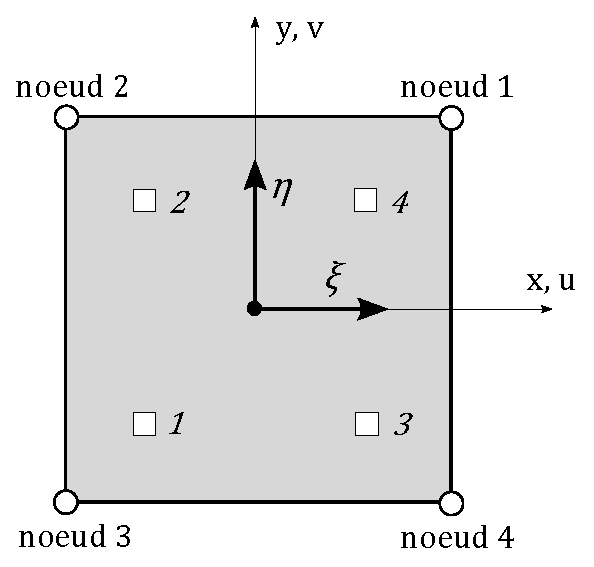
\includegraphics[height=50mm]{ptGauss} 
\caption{Élément rectangulaire de référence~$Q_1$ avec quatre points de Gauß} 
\label{ptGauss}
\end{figure} 
%%%%----------------------------------------------------------
\subsection*{Intégration sur des carrés ou des cubes} 
%%%%----------------------------------------------------------
Sur les carrés et les cubes, qui correspondent à ce qui nous intéresse en terme d'éléments de référence, on obtient les formules suivantes: 
\begin{align}
&\int_{-1}^{-1}\int_{-1}^{-1} f(x,y)\d x\d y \approx \dsum_{i=1}^{n_x}\dsum_{j=1}^{n_y} \varpi_i\varpi_j f(x_i,x_j)\\
&\int_{-1}^{-1}\int_{-1}^{-1}\int_{-1}^{-1} f(x,y,z)\d x\d y\d z \approx \dsum_{i=1}^{n_x}\dsum_{j=1}^{n_y}\dsum_{k=1}^{n_z} \varpi_i\varpi_j\varpi_k f(x_i,x_j,x_k)
\end{align}
où~$n_x$, $n_y$ et~$n_z$ sont les nombres de points de Gauß utilisés dans les directions~$x$, $y$ et~$z$. Dans la pratique, on a souvent~$n_x=n_y=n_z$. 
%%%%----------------------------------------------------------
\subsection*{Intégration sur un triangle ou un tétraèdre} 
%%%%----------------------------------------------------------
Malheureusement, tous les éléments ne sont pas des segments, carrés ou cubes... on a également souvent à faire à des triangles et à des tétreèdres. Dans ce cas, on construit des formules spécifiques qui ne sont pas issues du cas monodimensionel. L'élément triangulaire de référence est un triangle isocèle côtés égaux de longueur 1. L'angle droit est à l'origine du repère. La forme générale d'intégration est: 
\begin{equation}
 I=\int_{\hat{K}} f(x,y)\d x\d y \approx \sum_{i=1}^n \varpi_if(x_i,y_i) 
\end{equation}
Les positions et poids des~$n$ points de Gauß\index[aut]{Gauß (Johann Carl Friedrich), 1777-1855, Allemand} sont choisis afin d'intégrer exactement un polynôme de degré~$N$. Le tout est listé dans le tableau~\ref{tab:IntNum:TriGauss}.
\begin{table}[ht]\centering
\begin{tabular}{cccccc} &~$n$ &~$x_i$ &~$y_i$ &~$\varpi_i$ &~$N$\\ \hline 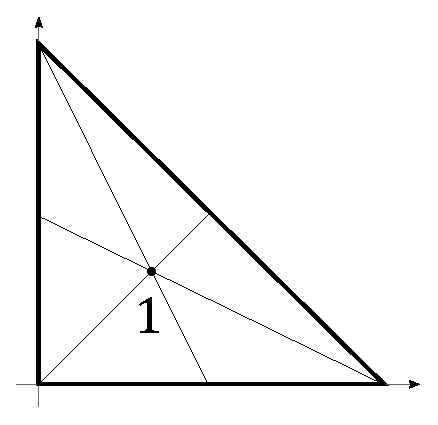
\includegraphics[height=30mm]{trG1} & 1 & 1/3 & 1/3 & 1/2 & 1\\ \hline \multirow{3}{*}{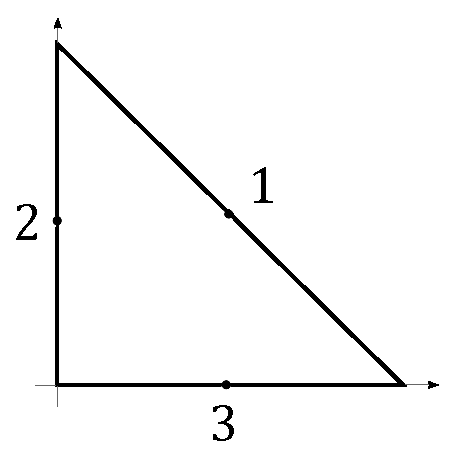
\includegraphics[width=30mm]{trG2}} & \multirow{3}{*}{3} & 1/2 & 1/2 & \multirow{3}{*}{1/6} & \multirow{3}{*}{2}\\[+2mm] &&0&1/2&&\\[+2mm] &&1/2&0&&\\[+12mm] \hline \multirow{3}{*}{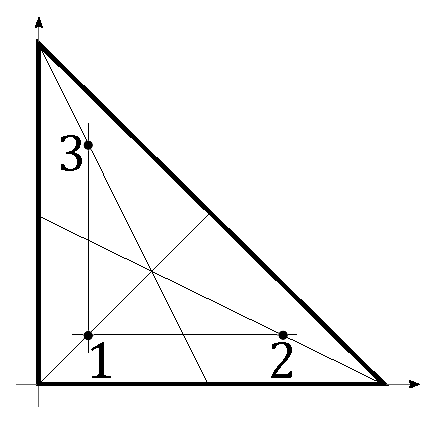
\includegraphics[height=30mm]{trG3}} & \multirow{3}{*}{3} & 1/6 & 1/6 & \multirow{3}{*}{1/6} & \multirow{3}{*}{2}\\[+2mm] &&2/3 & 1/6 &&\\[+2mm] &&1/6&2/3&&\\[+12mm] \hline \multirow{4}{*}{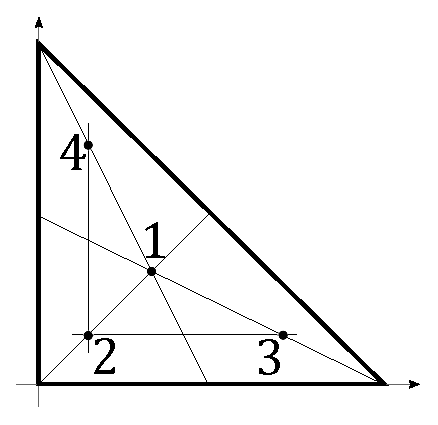
\includegraphics[height=30mm]{trG4}} & \multirow{4}{*}{4} & 1/3 & 1/3 & -27/96 & \multirow{3}{*}{4}\\[+2mm] &&1/5&1/5&25/96&\\[+2mm] &&3/5&1/5&25/96&\\[+2mm] &&1/5&3/5&25/96&\\[+12mm] 
\end{tabular} 
\caption{Triangles et points de Gauß}\label{tab:IntNum:TriGauss}
\end{table} 
 Le même travail peut être fait sur un tétraèdre. 